\documentclass[a4paper,11pt]{article}
\usepackage[portuguese]{babel}
\usepackage{graphicx}
\usepackage{amsmath}
\usepackage{minted}
\usepackage{mdframed}
\usepackage[all]{xy}

\usepackage[twoside,verbose,body={16cm,24cm},
left=25mm,top=20mm]{geometry}


\title{Cálculo de Programas \\ Resolução - Ficha 03}
\author{Eduardo Freitas Fernandes}
\date{2025}

\setminted{
	frame=single,
	tabsize=4,
	breaklines=true
}


\begin{document}
	
	\maketitle
	
	\noindent \underline{\textbf{Exercício 1}}
	\begin{center}
		\begin{minipage}{0.6\textwidth}
			\begin{mdframed}
				\[
				\begin{aligned}
					&\equiv \{\text{def. assocl, Fusão-$\times$, Reflexão-$\times$, Eq-$\times$}\}\\
					&\equiv \{\text{Def-$\times$, Universal-$\times$}\}\\
					&\equiv \{\text{associação à direita}\}\\
					&\equiv \{\text{Universal-$\times$}\}\\
					&\equiv \{\text{Natural-id, Universal-$\times$}\}
				\end{aligned}
				\]
			\end{mdframed}
		\end{minipage}
	\end{center}
	
	
	\noindent \underline{\textbf{Exercício 2}}
\begin{verbatim}
ghci> assocr = split (p1 . p1) (p2 >< id)
ghci> :t assocr
assocr :: ((b1, b2), d) -> (b1, (b2, d))
ghci> assocr ((3,4), 5)
(3,(4,5))
ghci> assocr ((x,y), z) = (x, (y,z))
ghci> :t assocr
assocr :: ((a1, a2), b) -> (a1, (a2, b))
ghci> assocr ((3,4), 5)
(3,(4,5))
\end{verbatim}
	
	
	\noindent \underline{\textbf{Exercício 3}}
	
	
	\begin{minipage}{0.3\textwidth}
		\[
		\frac{
			\begin{array}{c}
				f: A \rightarrow B \\
				g: C \rightarrow D
			\end{array}
		}{
			f \times g: A \times C \rightarrow B \times D
		}
		\]
	\end{minipage}
	\hfill
	\begin{minipage}{0.3\textwidth}
		\[
		\frac{
			\begin{array}{c}
				f: A \rightarrow B \\
				g: A \rightarrow C
			\end{array}
		}{
			\langle f, g \rangle : A \rightarrow B \times C
		}
		\]
	\end{minipage}
	\hfill
	\begin{minipage}{0.3\textwidth}
		\[
		\frac{
			\begin{array}{c}
				f: A \rightarrow B \\
				g: B \rightarrow C
			\end{array}
		}{
			f \cdot g: A \rightarrow C
		}
		\]
	\end{minipage}
	
	\begin{minipage}{0.45\textwidth}
		\[
		\frac{
			\begin{array}{c}
				\pi_2: A \times B \rightarrow B \\
				\pi_1: A \times B \rightarrow A
			\end{array}
		}{
			\langle \pi_2, \pi_1 \rangle : A \times B \rightarrow B \times A
		}
		\]
	\end{minipage}
	\hfill
	\begin{minipage}{0.45\textwidth}
		\[
		\frac{
			\begin{array}{c}
				id: A \rightarrow A \\
				swap: B \times C \rightarrow C \times B
			\end{array}
		}{
			id \times swap: A \times (B \times C) \rightarrow A \times (C \times B)
		}
		\]
	\end{minipage}
	\\
	
	\[
		\frac{
			\begin{array}{c}
				swap: D \times E \rightarrow E \times D \\
				id \times swap: A \times (B \times C) \rightarrow A \times (C \times B)
			\end{array}
		}{
			swap \cdot (id \times swap): A \times (B \times C) \rightarrow (C \times B) \times A
		}
	\]
	
	\newpage
	
	\[
	\begin{aligned}
		&\beta\cdot (f \times (g \times h)) \\
		= \  &\{\text{def. $\beta$}\}\\
		& swap \cdot (id \times swap) \cdot (f \times (g \times h)) \\
		= \  &\{\text{(F0)}\}\\
		& (id \times swap) \cdot swap \cdot (f \times (g \times h)) \\
		= \  &\{\text{(F0)}\}\\
		& (swap \times id) \cdot ((g \times h) \times f) \cdot swap \\
		= \  &\{\text{Functor-$\times$}\}\\
		& ((swap \cdot (g \times h)) \times (id \cdot f)) \cdot swap\\
		= \  &\{\text{(F0)}\}\\
		& (((h \times g) \cdot swap) \times (f \cdot id)) \cdot swap \\
		= \  &\{\text{Functor-$\times$}\}\\
		& ((h \times g) \times f) \cdot (swap \times id) \cdot swap \\
		= \  &\{\text{(F0)}\}\\
		& ((h \times g) \times f) \cdot swap \cdot (id \times swap) \\
		= \  &\{\text{def. $\beta$}\}\\
		& ((h \times g) \times f) \cdot \beta
	\end{aligned}
	\]
	
	\noindent \underline{\textbf{Exercício 4}}\\
	\[
	\underline{k} \ x = \underline{k} \ (x) = \underline{k} \ (id \ x) = \underline{k} \cdot id = \underline{k} = k
	\]
	
	\noindent \underline{\textbf{Exercício 5}}
	
\begin{verbatim}
ghci> data X = B Bool | P (Bool,Int)
ghci> :t B
B :: Bool -> X
ghci> :t P
P :: (Bool, Int) -> X
ghci> f = either B P
ghci> :t f
f :: Either Bool (Bool, Int) -> X
\end{verbatim}
	
	\noindent \underline{\textbf{Exercício 6}}\\
	
	\begin{minipage}{0.5\textwidth}
		\[
		\frac{
			\begin{array}{c}
				\underline{False}: A \rightarrow Bool \\
				id: A \rightarrow A
			\end{array}
		}{
			\langle \underline{False}, id \rangle : A \rightarrow Bool \times A
		}
		\]
	\end{minipage}
	\hfill
	\begin{minipage}{0.5\textwidth}
		\[
		\frac{
			\begin{array}{c}
				f: A \rightarrow C \\
				g: B \rightarrow C
			\end{array}
		}{
			[f, g]: A + B \rightarrow C
		}
		\]
	\end{minipage}\\
	
	
		\[
		\frac{
			\begin{array}{c}
				\langle \underline{False}, id \rangle : A \rightarrow Bool \times A \\
				\langle \underline{True}, id \rangle : A \rightarrow Bool \times A
			\end{array}
		}{
			[\langle \underline{False}, id \rangle, \langle \underline{True}, id \rangle]: A + A \rightarrow Bool \times A
		}
		\]
	
	
	\newpage
	
	\noindent \underline{\textbf{Exercício 7}}\\
	
	\[
	\begin{aligned}
		&\alpha = \ [\langle \underline{False}, id \rangle, \langle \underline{True}, id \rangle] \\
		\equiv \  &\{\text{Universal-+}\}\\
		&\begin{cases}
			\alpha \cdot i_1 = \langle \underline{False}, id \rangle \\
			\alpha \cdot i_2 = \langle \underline{True}, id \rangle
		\end{cases}\\
		\equiv \  &\{\text{point wise}\}\\
		&\begin{cases}
			(\alpha \cdot i_1) \ a = \langle \underline{False}, id \rangle \ a \\
			(\alpha \cdot i_2) \ a = \langle \underline{True}, id \rangle \ a
		\end{cases}\\
		\equiv \  &\{\text{def. composição, def. split}\}\\
		&\begin{cases}
			\alpha (i_1 \ a) = (\underline{False} \ a, id \ a) \\
			\alpha (i_2 \ a) = (\underline{True} \ a, id \ a)
		\end{cases}\\
		\equiv \  &\{\text{def. const, def. id}\}\\
		&\begin{cases}
			\alpha (i_1 \ a) = (False, a) \\
			\alpha (i_2 \ a) = (True, a)
		\end{cases}\\
	\end{aligned}
	\]
	
\begin{verbatim}
ghci> alpha (Left a) = (False, a)
ghci> alpha (Right a) = (True, a)
\end{verbatim}
	
	\noindent \underline{\textbf{Exercício 8}}\\
	
	\begin{minipage}{0.5\textwidth}
		\[
		\frac{
			\begin{array}{c}
				\pi_1: A \times B \rightarrow A \\
				id: C \rightarrow C
			\end{array}
		}{
			\pi_1 \times id: (A \times B) \times C \rightarrow A \times C
		}
		\]
	\end{minipage}
	\hfill
	\begin{minipage}{0.5\textwidth}
		\[
		\frac{
			\begin{array}{c}
				\pi_2: A \times B \rightarrow B \\
				\pi_1: (A \times B) \times C \rightarrow A \times B
			\end{array}
		}{
			\pi_2 \cdot \pi_1: (A \times B) \times C \rightarrow B
		}
		\]
	\end{minipage}\\
	
	
	\[
	\frac{
		\begin{array}{c}
			\pi_1 \times id: (A \times B) \times C \rightarrow A \times C \\
			\pi_2 \cdot \pi_1: (A \times B) \times C \rightarrow B
		\end{array}
	}{
		\langle \pi_1 \times id, \pi_2 \cdot \pi_1 \rangle: (A \times B) \times C \rightarrow (A \times C) \times B
	}
	\]
	
	
	\[
	\begin{aligned}
		& xr \cdot \langle \langle f, g \rangle , h \rangle = \langle \langle f, h \rangle , g \rangle \\
		\equiv \  &\{\text{Universal-$\times$}\}\\
		&\begin{cases}
			\pi_1 \cdot xr \cdot \langle \langle f, g \rangle , h \rangle = \langle f, h \rangle \\
			\pi_2 \cdot xr \cdot \langle \langle f, g \rangle , h \rangle = g
		\end{cases}\\
		\equiv \  &\{\text{def. xr, Cancelamento}\}\\
		&\begin{cases}
			(\pi_1 \times id) \cdot \langle \langle f, g \rangle , h \rangle = \langle f, h \rangle \\
			\pi_2 \cdot \pi_1 \cdot \langle \langle f, g \rangle , h \rangle = g
		\end{cases}\\
		\equiv \  &\{\text{Absorção-$\times$, Cancelamento-$\times$}\}\\
		&\begin{cases}
			\langle \pi_1 \cdot \langle f, g \rangle, id \cdot h \rangle = \langle f, h \rangle \\
			\pi_2 \cdot \langle f, g \rangle = g
		\end{cases}\\
		\equiv \  &\{\text{Cancelamento-$\times$}\}\\
		&\begin{cases}
			\langle f, h \rangle = \langle f, h \rangle \\
			g = g
		\end{cases}\\
	\end{aligned}
	\]
	
	
	\newpage
	
	\noindent \underline{\textbf{Exercício 9}}\\
	
\begin{minted}{haskell}
mkInd :: (Bib, Aux) -> Ind
mkInd = map (id >< sort) 
		. uncurry applyMapping 
		. swap 
		. (invertRelation >< invertRelation)

invertRelation :: (Ord a, Ord b) => [(a, [b])] -> [(b, [a])]
invertRelation = groupPairs . sortOn p1 . map swap . expandPairs

expandPairs :: [(a, [b])] -> [(a, b)]
expandPairs = concat . map (\(x, l) -> map (x,) l)

groupPairs :: (Eq a) => [(a, b)] -> [(a, [b])]
groupPairs = uncurry zip . split
							(nub . map p1)
							(map (map p2) 
							 . groupBy (curry (uncurry (==) 
							 		           . (p1 >< p1))))

applyMapping :: (Eq b) => [(b, [c])] -> [(a, [b])] -> [(a, [c])]
applyMapping a = map (applyMappingOne a)

applyMappingOne :: (Eq b) => [(b, [c])] -> (a, [b]) -> (a, [c])
applyMappingOne d = id >< (concat . map ( \x -> case lookup x d of 
													Just xs -> xs
													_ -> []))
\end{minted}
	
\begin{figure}[H]
	\centering
	\fbox{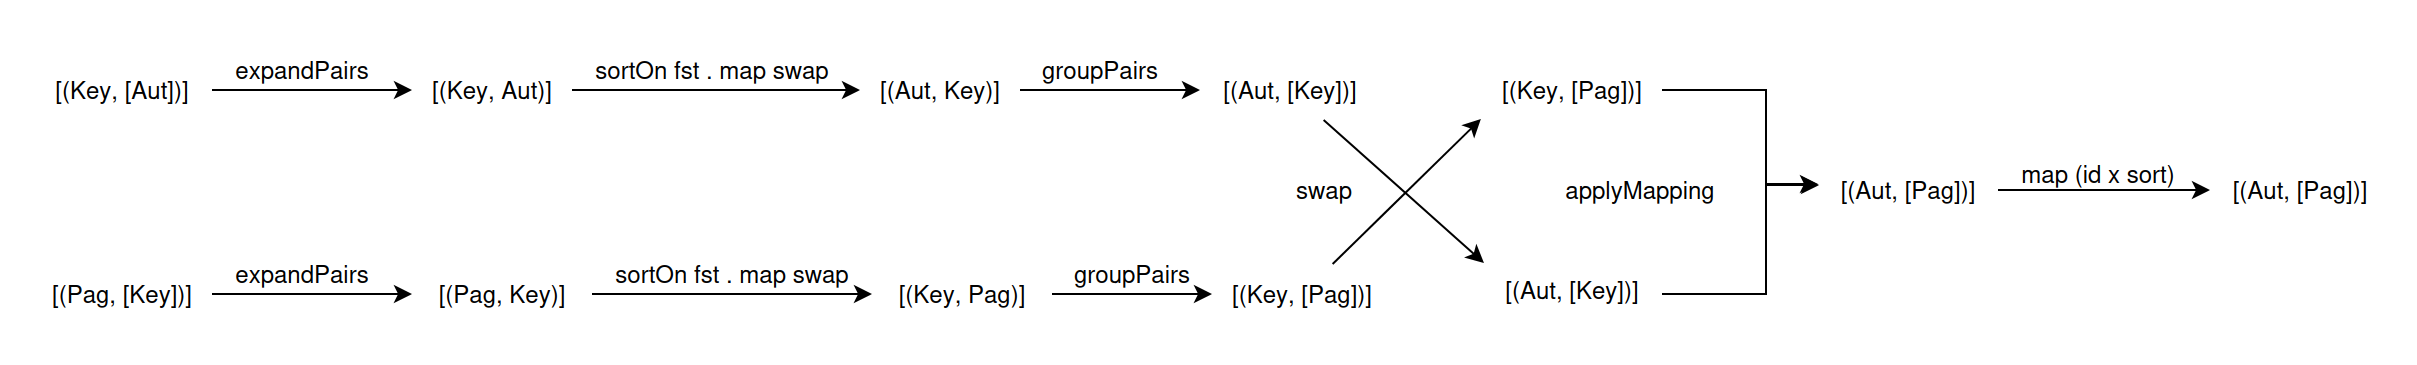
\includegraphics[width=1\textwidth]{qp-f3.png}}
	\caption{mkInd}
\end{figure}
	
\end{document}
